%===============================================================================
% Autorka: Bc. Eva Navrátilová
% Kontakt: xnavra54@stud.fit.vutbr.cz, navratie@gmail.com
%===============================================================================

% Tento soubor nahraďte vlastním souborem s přílohami (nadpisy níže jsou pouze pro příklad)
% This file should be replaced with your file with an appendices (headings below are examples only)

% Umístění obsahu paměťového média do příloh je vhodné konzultovat s vedoucím
% Placing of table of contents of the memory media here should be consulted with a supervisor
%\chapter{Obsah přiloženého paměťového média}

%\chapter{Manuál}

%\chapter{Konfigurační soubor} % Configuration file

\chapter{Obsah přiloženého paměťového média}
	\label{append:cd}
	\begin{itemize}
		\item \texttt{readme.txt}~--~Obsahuje informace o~aplikaci, instalaci a~repozitáři
		\item \texttt{doc/}
		\begin{itemize}
			\item \texttt{thesis/}~--~Text této práce a~latexové zdrojové kódy
			\item \texttt{doxygen/}~--~Dokumentace kódu vygenerovaná prostřednictvím Doxygenu
			\item \texttt{tutorial/}~--~Obrázkový návod k~použití aplikace
		\end{itemize}
		\item \texttt{src/}~--~Makefile
		\begin{itemize}
			\item \texttt{src/}~--~Zdrojové kódy aplikace a~knihoven třetích stran
			\begin{itemize}
				\item \texttt{3rd-party/}~--~Zdrojové kódy použitých externích knihoven
				\item \texttt{kernel/}~--~Zdrojové kódy jádra aplikace
				\item \texttt{userinterface/}~--~Zdrojové kódy uživateslkého rozhraní aplikace
				\item \texttt{language/}~--~Překlady aplikace do přiřozených jazyků
			\end{itemize}
			\item \texttt{test/}~--~Zdrojové kódy automatických testů aplikace
		\end{itemize}
		\item \texttt{bin/}~--~Binární soubory
		\begin{itemize}
			%\item \texttt{linux/}~--~Spustitelný soubor pro linux (generuje se příkazem \texttt{make} v~\texttt{src/})
			\item \texttt{windows/}~--~Spustitelný .exe soubor pro Windows
		\end{itemize}
	\end{itemize}


\chapter{Plakát} % poster
\newpage
\label{append:poster}
\begin{figure}[H]
	\centering
	\includegraphics[width=15cm]{28_poster.pdf}
	\caption{Plakát využitý při účasti na konfercenci Excel@FIT}
\end{figure}


\chapter{Diagram tříd jádra aplikace}
\label{append:designKernel}
\begin{figure}[H]
	\centering
	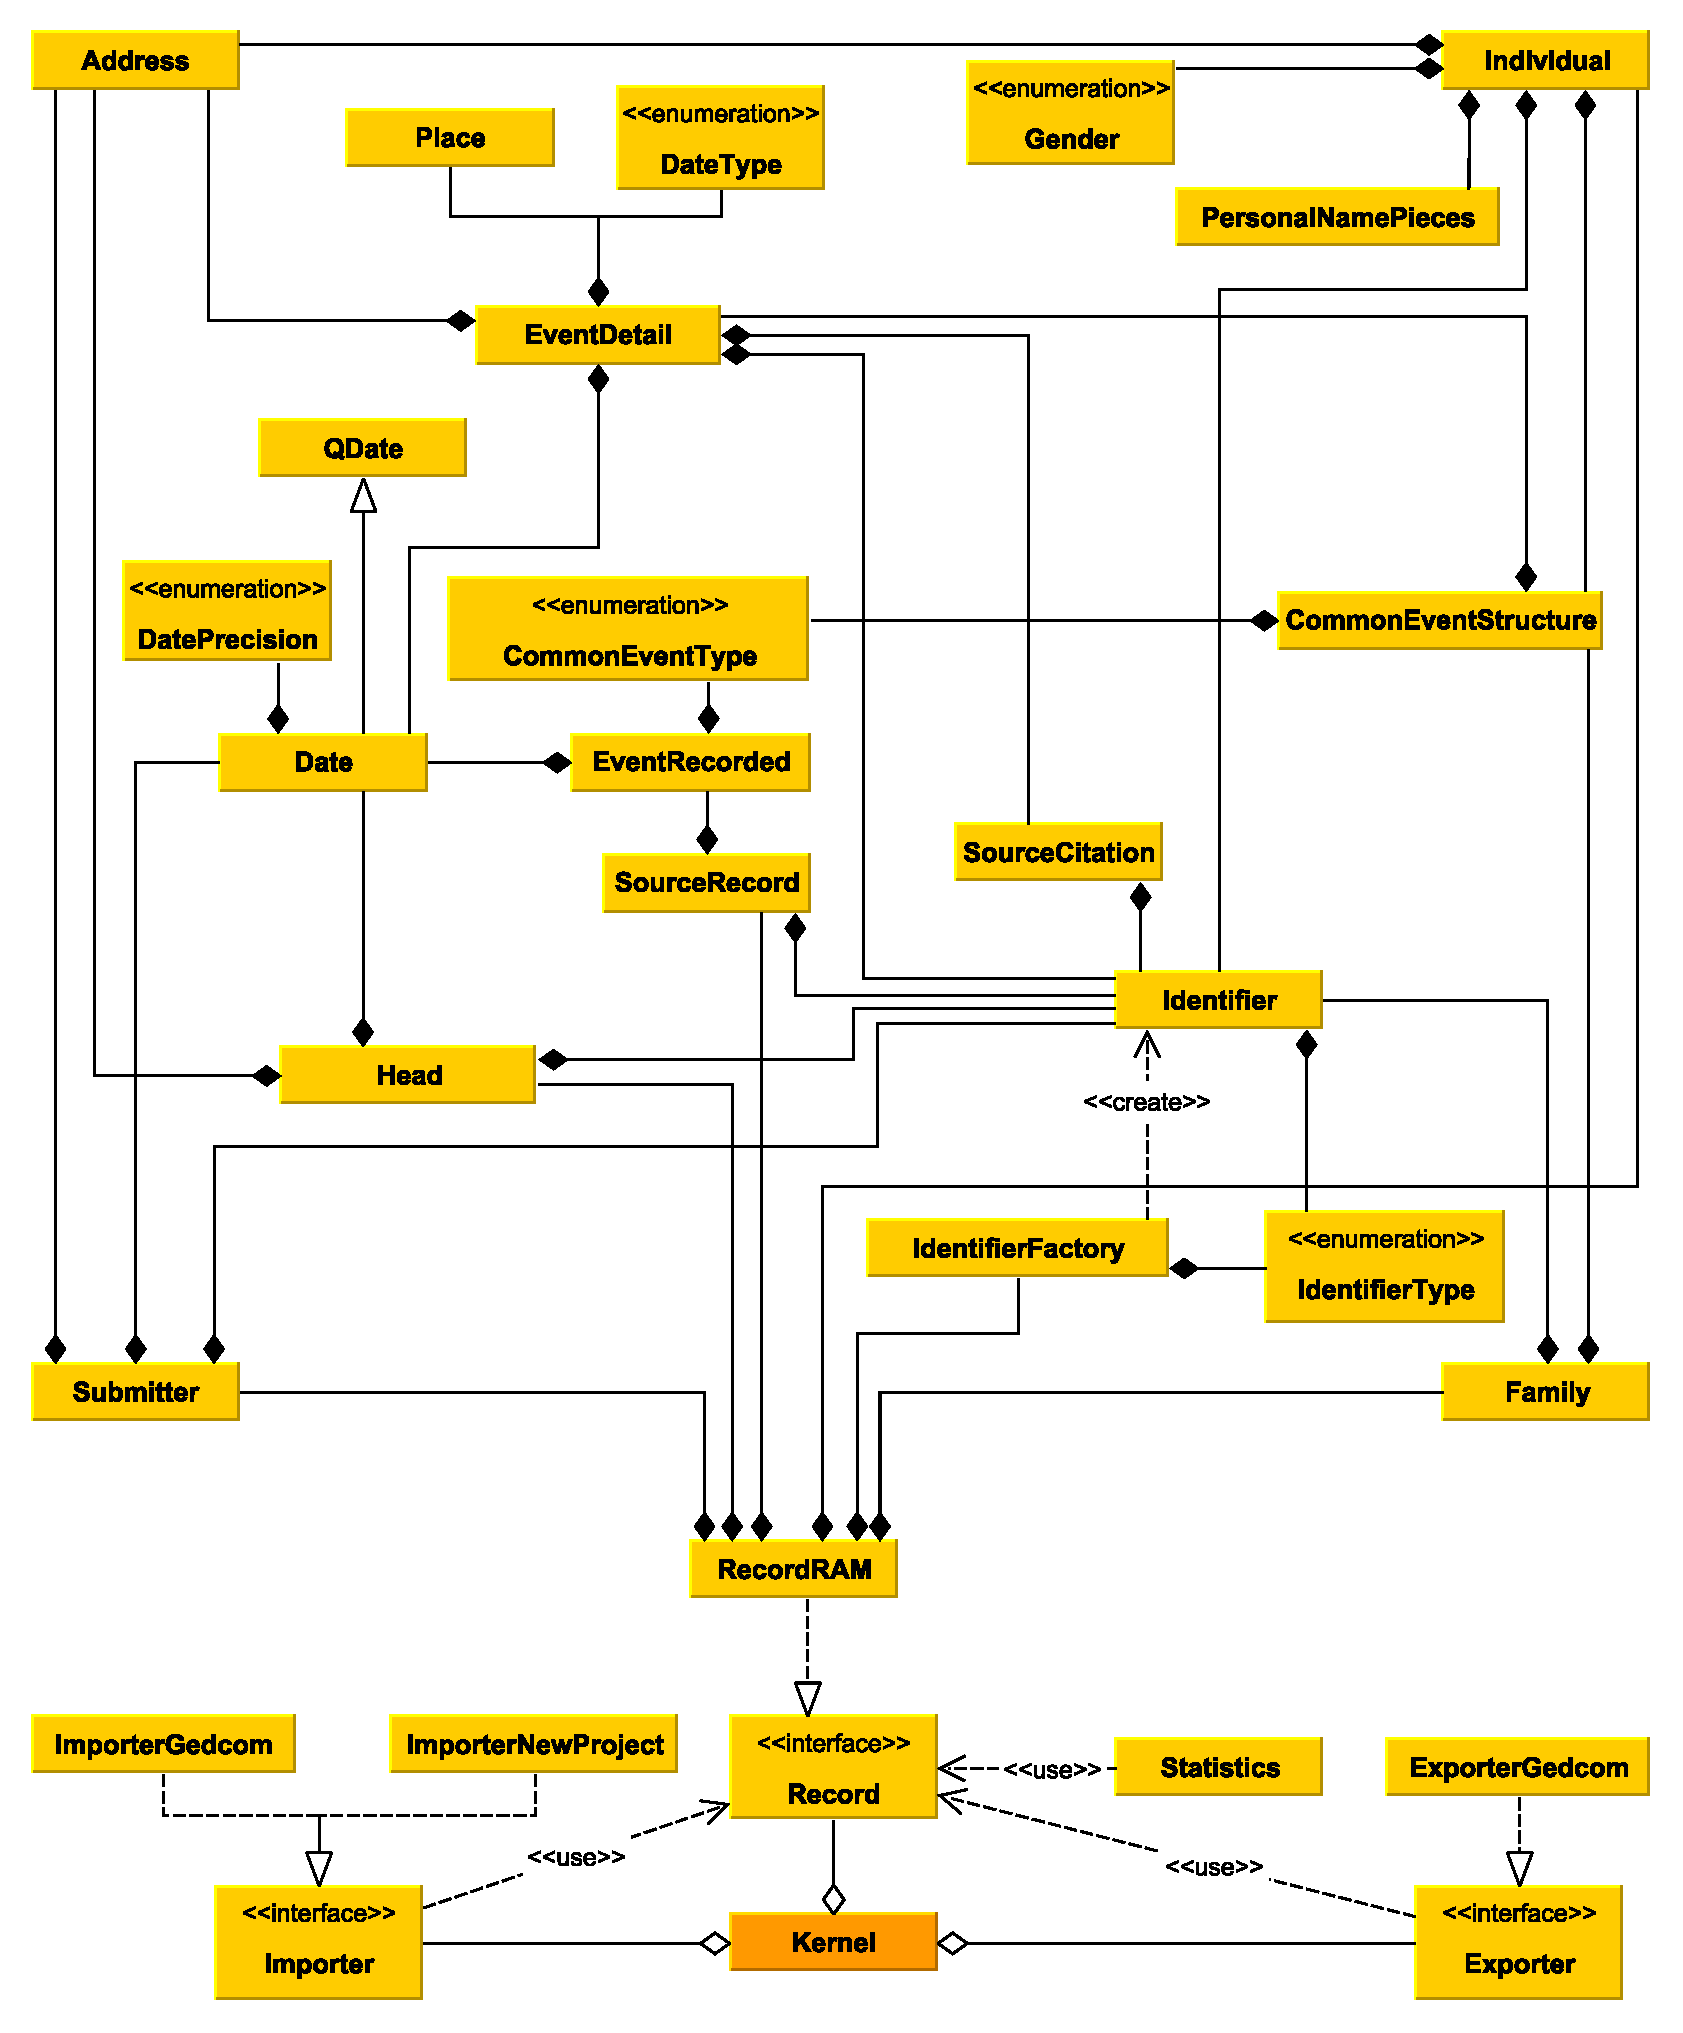
\includegraphics[width=13cm]{design/programFullClassOnly.pdf}
	\caption{Diagram tříd jádra aplikace}
\end{figure}




\chapter{Vzory formulářů}
	\section{Zkušenosti s genealogickými aplikacemi}
		\label{append:formZkusenosti}
		\subsection*{Jak dlouho pracujete s genealogickými programy?}
		\begin{itemize}
			\item[$\circ$] Méně než rok
			\item[$\circ$] 1 až 2 roky
			\item[$\circ$] 2 až 6 let
			\item[$\circ$] více než 6 let
		\end{itemize}
		\subsection*{Jaký genealogický program aktuálně používáte?}
		\dotfill
		\subsection*{Proč jste si tento program vybrali?}
		\dotfill
		\subsection*{Co vám na programu vyhovuje?}
		\dotfill
		\subsection*{Co vám v programu chybí, co byste na něm změnili?}
		\dotfill
		\subsection*{Zaznamenáváte u osob zdroje informací?}
		\begin{itemize}
			\item[$\circ$] Vždy
			\item[$\circ$] Občas
			\item[$\circ$] Nikdy
		\end{itemize}
		\subsection*{Jakým způsobem zdroje informací ukládáte do programu?}
		\begin{itemize}
			\item[$\square$] Webový odkaz na digitalizovanou stránku matriky, kde se nachází záznam o předkovi
			\item[$\square$] Signatura matriky, číslo stránky
			\item[$\square$] Zaznamenávám i pozici zápisu na stránce
			\item[$\square$] \dotfill
		\end{itemize}
		\subsection*{Vaše poznámky}
		\dotfill

	\newpage
	\section{Hodnocení aplikace ProGenealogy}
		\label{append:formHodnoceni}
		\subsection*{Jakou aplikaci aktuálně používáte?}
		\begin{itemize}
			\item[$\square$] MyHeritage (Webové rozhraní)
			\item[$\square$] Ancestry
			\item[$\square$] MyHeritage FamilyTreeBuilder
			\item[$\square$] \dotfill
		\end{itemize}
		\subsection*{Jaké jsou vaše dojmy z aplikace ProGenealogy?}
		\dotfill
		\subsection*{Jak se vám aplikace ovládala?}
		Výborně    \quad $\circ$ $\circ$ $\circ$ $\circ$ $\circ$ $\circ$ \quad Špatně
		\subsection*{Uvažovali byste o přechodu na tuto aplikaci?}
		Určitě ano \quad $\circ$ $\circ$ $\circ$ $\circ$ $\circ$ $\circ$ \quad Určitě ne
		\subsection*{Co se vám na aplikaci líbí?}
		\dotfill
		\subsection*{Co byste na aplikaci změnili?}
		\dotfill
		\subsection*{Co vám v aplikaci chybí? Co byste přidali?}
		\dotfill
		\subsection*{Co bylo v aplikaci zbytečné? Co byste odebrali?}
		\dotfill
		\subsection*{Jak dlouho jste s aplikací ProGenealogy pracovali?}
		\begin{itemize}
			\item[$\circ$] méně než 10 minut
			\item[$\circ$] 10 až 30 minut
			\item[$\circ$] 30 minut až 1 hodinu
			\item[$\circ$] více než 1 hodinu
		\end{itemize}
	
	



